\section{Forforstærker}

\begin{frame}{Forforstærker}
\begin{itemize}
\item Forstærke signal fra mikrofon
\item Mikrofon: MCE-4000
\item Mikrofons output spænding: 0,8 - 200 mV
\item Output som skal opnås: 200 mV - 2 V
\item Lineær forstærkning ikke muligt
\item Valgte peakspændinger beregnet ud fra forventeligt lydtryk
\end{itemize}
\end{frame}

\begin{frame}{Forforstærker - Krav}

\scriptsize{\begin{table}[h]
\centering
\begin{tabular}{l|r}
\hline\hline
Område & Krav \\
\hline\hline
Indgangsimpedans & 22 k\ohm \\[4pt]
Frekvensgang & \< 0,375 dB ved 20 Hz - 20 kHz, ref. 1 kHz \\
& \< 0,75 dB fra 20 Hz til 63 Hz \\
& \< 0,75 dB fra 12,5 kHz til 20 kHz \\[4pt]
Forvrængning & \< 0,5 \% \\[4pt]
Forstærkning & 69,7 gange ved 22 k\ohm~ indgangsimpedans og ved 1 kHz \\
\hline\hline
\end{tabular}
\end{table}}

\end{frame}

\begin{frame}{Forforstærker - Opbygning}
\begin{itemize}
\item To common-emitter forstærkere med uafkoblet emittermodstand
\item Der vælges to trin for at opnå en stor mængde tilbagekobling
\item Trin 1: 10 ganges forstærkning
\item Trin 2: 6,97 ganges forstærkning
\end{itemize}
\end{frame}

\begin{frame}{Forforstærker - Accepttest}
\begin{itemize}
\item Indgangsimpedans målt til 22 k\ohm
\item Frekvensgang: 
\end{itemize}
\begin{figure}[h]
\centering
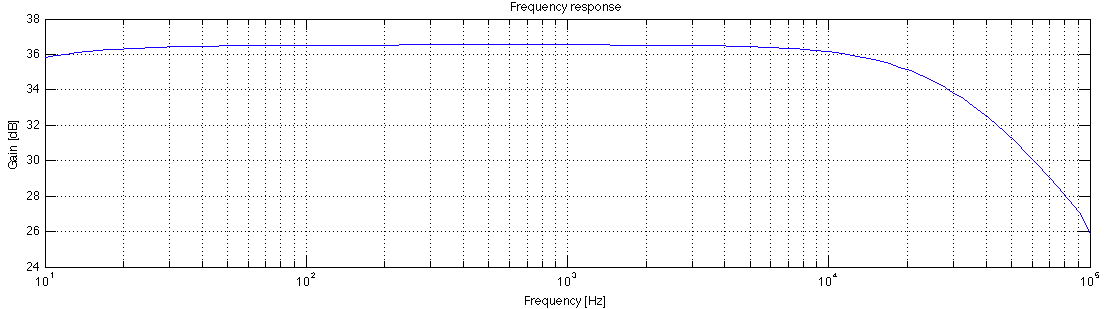
\includegraphics[scale=.25]{images/frekvensrespons-forforstaerker.png}
\end{figure}

\end{frame}

\begin{frame}{Forforstærker - Accepttest}
\begin{itemize}
\item Fra 20 Hz til 63 Hz
\end{itemize}
\begin{figure}[h]
\centering
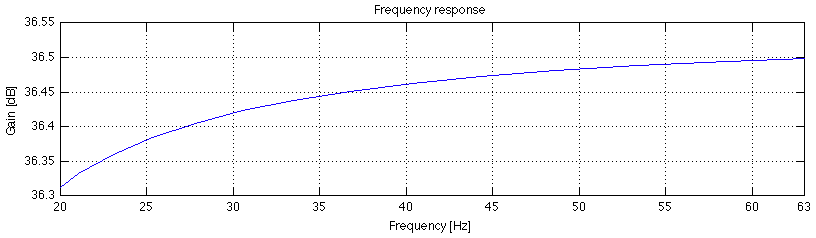
\includegraphics[scale=.3]{images/fr20-63.png}
\end{figure}
\end{frame}

\begin{frame}{Forforstærker - Accepttest}
\begin{itemize}
\item Fra 12 kHz til 20 kHz
\end{itemize}
\begin{figure}[h]
\centering
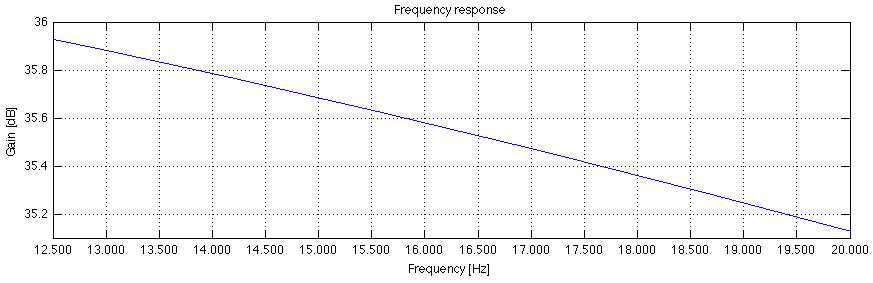
\includegraphics[scale=.3]{images/fr12-20k.png}
\end{figure}
\end{frame}

\begin{frame}{Forforstærker - Accepttest}

\scriptsize{\begin{table}[h]
\centering
\begin{tabular}{l|r|r}
\hline\hline
Område & Krav & Status \\
\hline\hline
Indgangsimpedans & 22 k\ohm & \checkmark\\[4pt]
Frekvensgang & \< 0,375 dB ved 20 Hz - 20 kHz, ref. 1 kHz & \checkmark\\
& \< 0,75 dB fra 20 Hz til 63 Hz & \checkmark\\
& \< 0,75 dB fra 12,5 kHz til 20 kHz & \checkmark \\[4pt]
Forvrængning & \< 0,5 \% & \checkmark\\[4pt]
Forstærkning & 69,7 gange ved 22 k\ohm~ & \checkmark\\
	&	indgangsimpedans og ved 1 kHz & \\
\hline\hline
\end{tabular}
\end{table}}

\end{frame}
